% This example is meant to be compiled with lualatex or xelatex
% The theme itself also supports pdflatex
\PassOptionsToPackage{unicode}{hyperref}
\documentclass[aspectratio=1610, 9pt, xcolor=dvipsnames]{beamer}
\usepackage[absolute,overlay]{textpos}
\usepackage{graphicx,caption}
\parskip0pt
% Load packages you need here
\usepackage{polyglossia}
\setmainlanguage{german}

\usepackage{csquotes}

\usepackage{tikz}

\usepackage{subfig}

\usepackage[export]{adjustbox}

\usepackage{amsmath}
\usepackage{amssymb}
\usepackage{mathtools}
\usepackage{unicode-math}
\usepackage{xfrac}

\usepackage{environ}

\usepackage{hyperref}
\usepackage{bookmark}
\usepackage{graphicx}
\usepackage{wrapfig}

\usepackage{booktabs}

\usepackage{multicol}

\usepackage{relsize}

\usepackage[dvipsnames]{xcolor}

\usepackage{bm}

\usepackage{empheq}
\newcommand*\widefbox[1]{\fbox{\hspace{2em}#1\hspace{2em}}}

\makeatletter
\newcommand{\Pause}[1][]{\unless\ifmeasuring@\relax
\pause[#1]%
\fi}
\makeatother

\usepackage[
locale=DE,
separate-uncertainty=true, % Immer Unsicherheit mit ±
per-mode=symbol-or-fraction, % m/s im Text, sonst \frac
% alternativ:
% per-mode=reciprocal, % m s^{-1}
% output-decimal-marker=., % . statt , für Dezimalzahlen
]{siunitx}

% load the theme after all packages

\usetheme[
  %showtotalframes, % show total number of frames in the footline
]{tudo}

% Put settings here, like
\unimathsetup{
  math-style=ISO,
  bold-style=ISO,
  nabla=upright,
  partial=upright,
  mathrm=sym,
}

\DeclarePairedDelimiter{\bra}{\langle}{\rvert}
\DeclarePairedDelimiter{\ket}{\lvert}{\rangle}
\DeclarePairedDelimiterX{\braket}[2]{\langle}{\rangle}{
#1 \delimsize| #2
}

\newenvironment<>{varblock}[2][.9\textwidth]{%
  \setlength{\textwidth}{#1}
  \begin{actionenv}#3%
    \def\insertblocktitle{#2}%
    \par%
    \usebeamertemplate{block begin}}
  {\par%
    \usebeamertemplate{block end}%
  \end{actionenv}}


\NewEnviron{myequation}{%
  \begin{equation*}
  \scalebox{1.5}{$\BODY$}
  \end{equation*}
}

%----------------------------------------
%Align Equations to LEFT MARGIN (use \mathleft then \mathcenter)
\makeatletter
\newcommand{\mathleft}{\@fleqntrue\@mathmargin0pt}
\newcommand{\mathcenter}{\@fleqnfalse}
\makeatother
%----------------------------------------

\title{Quantum annealing und Logistik}
\author[Y.~Kind]{Yanick Kind}
\institute[]{Fakultät Physik}
\date{12. Juli 2023}


\begin{document}

\maketitle

\begin{frame}{Übersicht}
  \begin{columns}
    \column{0.4\linewidth}
    \setlength{\parskip}{4ex}
    \tableofcontents
    \column{0.6\linewidth}
    \vspace*{1cm}
    \centering
    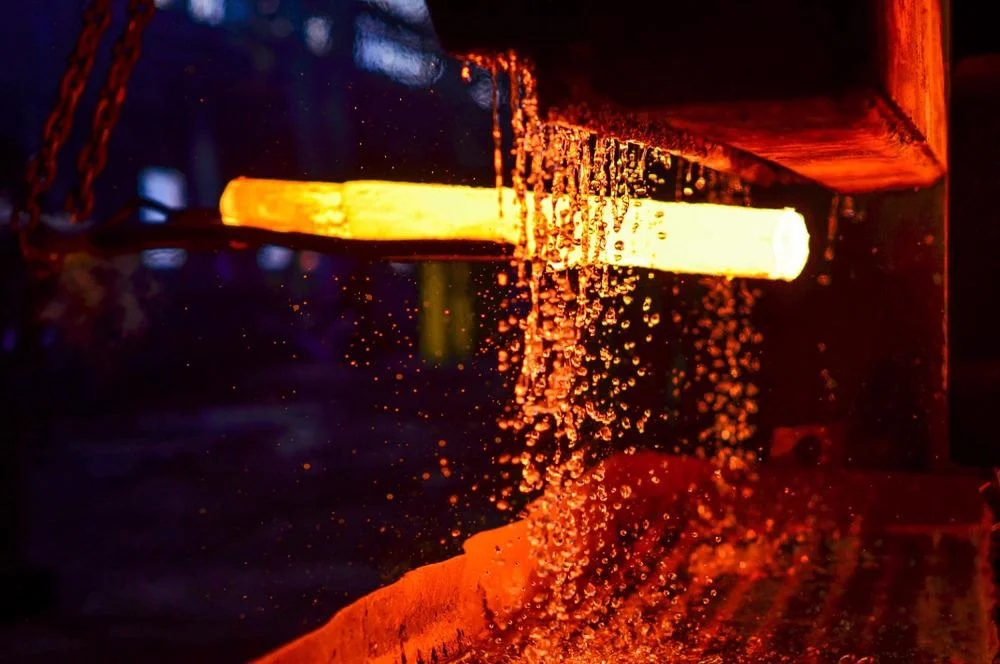
\includegraphics[width = \textwidth]{Plots/annealing_front.png}
    \hspace*{12pt}\hbox{\scriptsize {\footnotesize\itshape \href{https://www.azom.com/article.aspx?ArticleID=20342}{azom.com}}}
  \end{columns}
\end{frame}

\section{Einleitung}

\begin{frame}{Motivation}
  \centering
  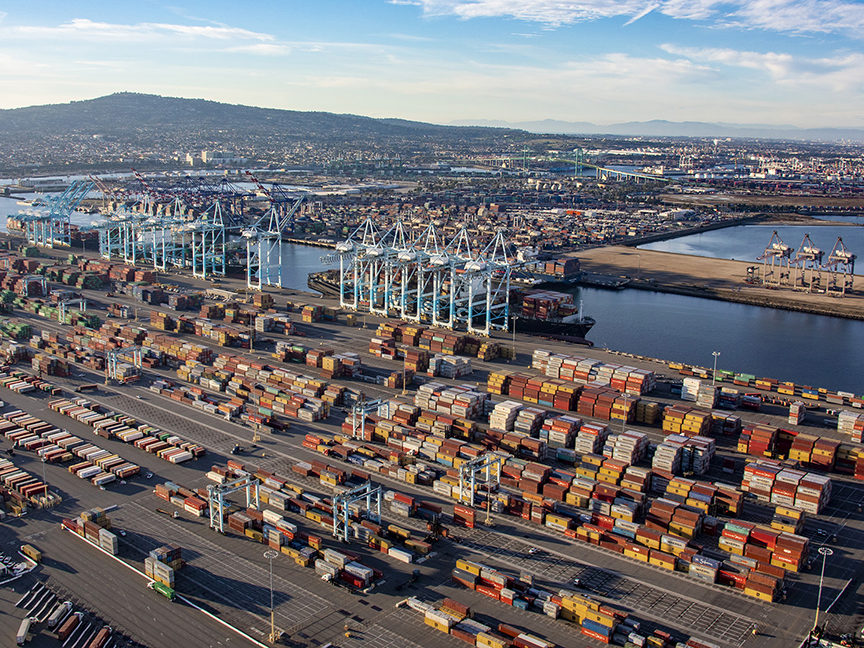
\includegraphics[width = 0.6\textwidth]{Plots/LA.jpg}\\
  \hspace*{12pt}\hbox{\scriptsize {\footnotesize\itshape \href{https://www.supplychainbrain.com/articles/35529-another-month-of-high-volume-at-port-of-los-angeles-while-exports-continue-to-fall}{supplychainbrain.com}}}
\end{frame}

\begin{frame}{Traveling Salesman Problem}
  \begin{textblock*}{7cm}(11cm, 1.6cm)
    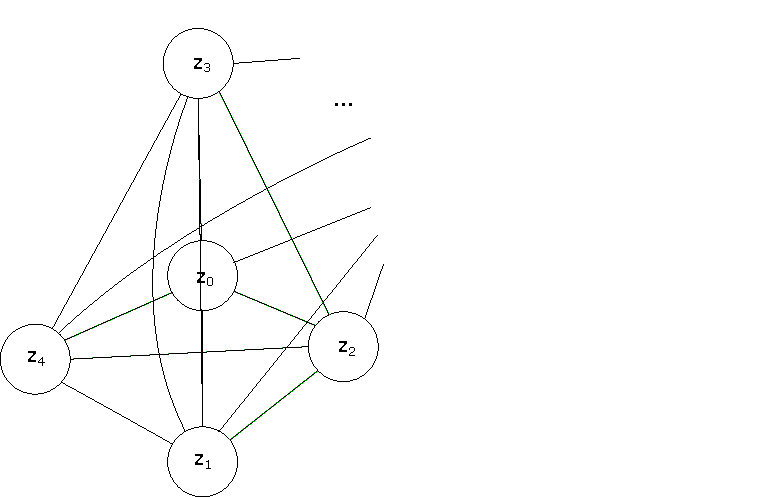
\includegraphics[width = \textwidth]{Plots/ex.pdf}
  \end{textblock*}
  \pause
  \begin{itemize}
    \setlength\itemsep{1em}
    \item klassisches kombinatorisches Optimierungsproblem
    \pause
    \item Beispiel: Ein Lieferwagen hat $n$ Lieferorte
    \pause
    \begin{itemize}
      \item[\textrightarrow] $(n-1)!$ verschiedene Routen
    \end{itemize}
    \pause
    \item NP-hard
    \begin{itemize}
      \item[\textrightarrow] skaliert nicht polynomiell sondern \textbf{exponentiell} mit Systemgröße \pause
    \end{itemize}
    \item Globales Optimum mittels numerischen Lösungsverfahren finden, ist extrem aufwändig
    \pause
    \item Local search Algorithmen als heuristische Näherungsverfahren nutzen
  \end{itemize}  
\end{frame}

\begin{frame}{Annealing als Lösung?}
  \begin{columns}
    \column{0.3\linewidth}
      \centering
      \visible<1->{
       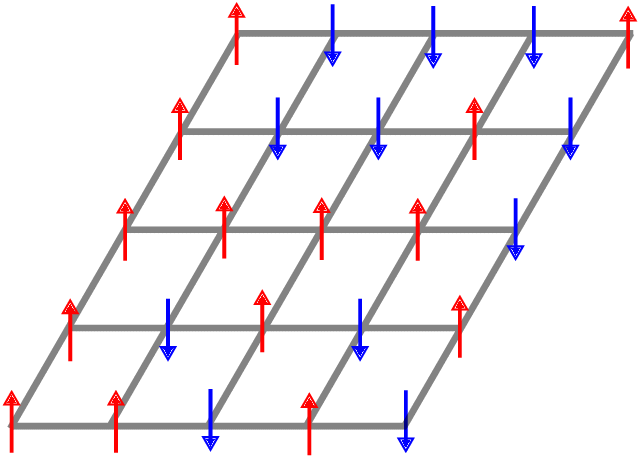
\includegraphics[width = 0.95\textwidth]{Plots/Ising_Modell_2d.png}
       \hspace*{12pt}\hbox{\scriptsize {\footnotesize\itshape \href{https://www.researchgate.net/publication/321920877_Thermalisation_and_Relaxation_of_Quantum_Systems}{Sascha Wald, Thermalisation and Relaxation of Quantum Systems (2017)}}}
      }\\ 
      \visible<2->{ \vspace*{1cm}
      \scalebox{3}{$E$}
      }
    \column{0.2 \linewidth}
    \centering  
      \vspace*{2.2cm}
      \visible<1->{\scalebox{4}{$\stackrel{?}{\to}$}}
    \column{0.3\linewidth}
     \centering
      \visible<1->{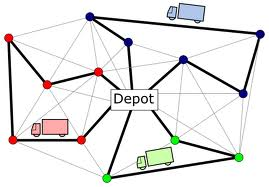
\includegraphics[width = 0.95 \textwidth]{Plots/vehicle_routing_problem.jpg}
      \hspace*{12pt}\hbox{\scriptsize {\footnotesize\itshape \href{https://www.r-bloggers.com/2010/11/any-r-packages-to-solve-vehicle-routing-problem/}{r-bloggers.com}}}
       } \\
     \vspace*{1cm}
     \visible<3->{
      \scalebox{3}{$f$}}
 \end{columns}
\end{frame}

\section{Simulated und quantum annealing}

\begin{frame}{Simulated annealing (SA)}
  \visible<1->{}
  \begin{itemize}
    \setlength\itemsep{1em}
    \visible<2->{\item in Analogie zu auskühlenden Metallen}
    \begin{itemize}
      \visible<3->{
      \pause
      \item schneller auskühlen \textrightarrow suboptimalerer Zustand (amorph)
      \pause
      \item langsamer auskühlen \textrightarrow optimalerer Zustand (kristallin) }
    \end{itemize}
    \visible<5->{
    \item nutzt thermische Fluktuationen, um lokalen Minima zu entkommen }
    \visible<6->{\item Wahrscheinlichkeit $P_i$ folgen Mastergleichung $\frac{dP_i}{dt} = \sum_j L_{ij} P_j$}
    \visible<7->{\begin{itemize}
      \item        $L_{ij} = 
      \begin{cases}
        \left [ 1 + \text{exp}((E_i -E_j) / T_t) \right ]^{-1}  & \, \text{einzelne Spin-Differenz} \\
        - \sum_{k \neq i} L_{ki}                                & \, i = j \\
        0                                                       & \, \text{sonst}
      \end{cases}
    $}
    \end{itemize}
  \end{itemize}
  \begin{textblock*}{6cm}(9.9cm,2.05cm) % {block width} (coords)
    \visible<5->{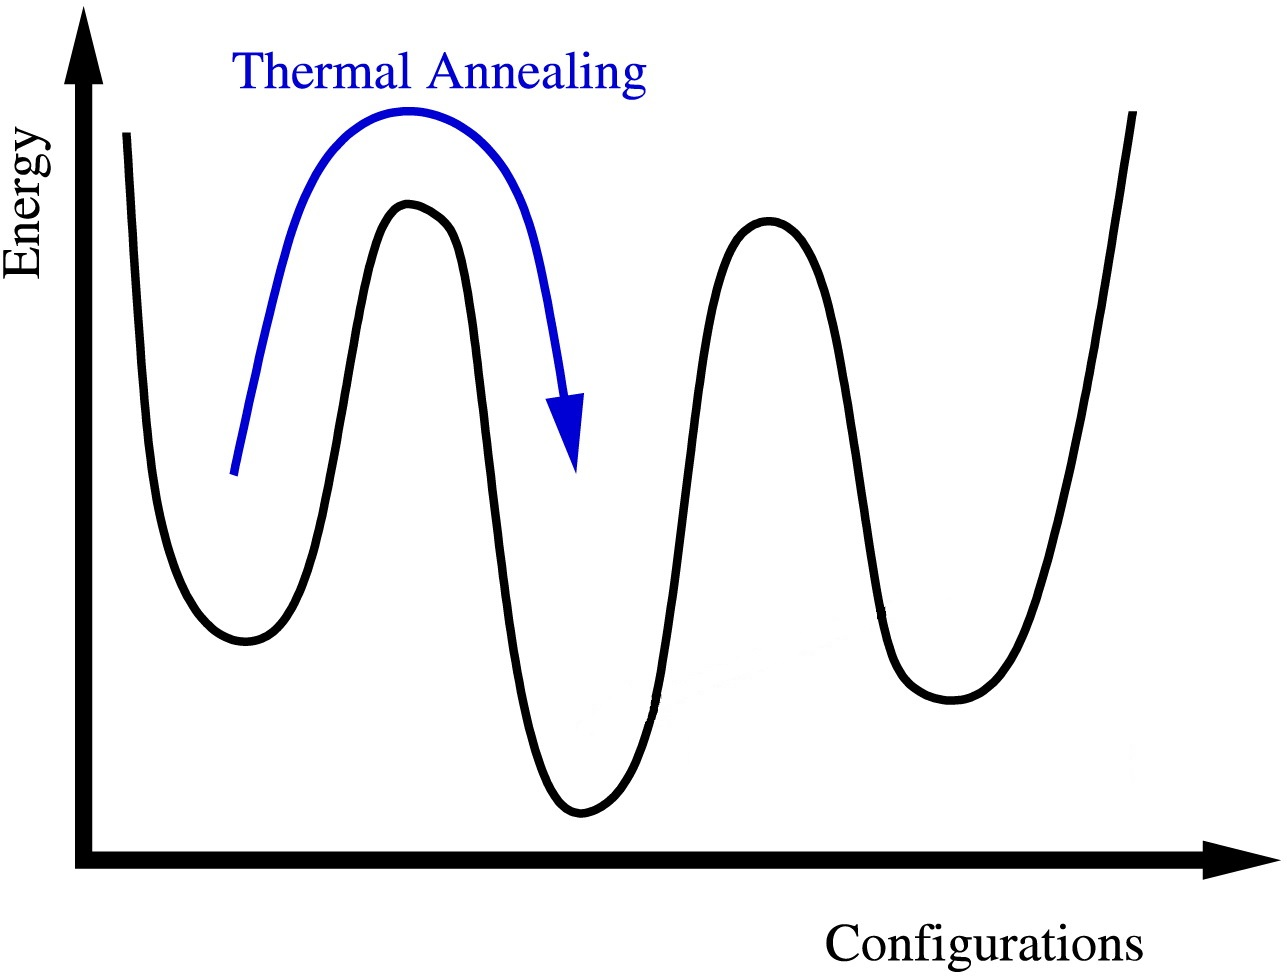
\includegraphics[width = 5cm]{Plots/thermal_annealing.jpg}
    \hspace*{12pt}\hbox{\scriptsize {\footnotesize\itshape \href{https://doi.org/10.1016/j.physrep.2012.10.002}{V. Bapst et al., \textit{Physics Reports} 523 (2013), editiert}}}
    }\end{textblock*}    
  \begin{textblock*}{6cm}(10cm,6.5cm) % {block width} (coords)
  \visible<4->{
\includegraphics[width = 5cm]{Plots/slow_fast_SA.png}
  \hspace*{12pt}\hbox{\scriptsize {\footnotesize\itshape \href{https://en.wikipedia.org/wiki/}{Cyp, wikipedia.org}}}}
  \end{textblock*}    
\end{frame}

\begin{frame}{Quantum Annealing (QA)}
  \visible<1->{}
  \begin{itemize}
    \setlength\itemsep{1em}
    \visible<2->{\item transversales Ising-Modell $H (t) = \underbrace{- \sum_{ij} J_{ij} \sigma_i^z \sigma_j^z - h \sum_i \sigma_i^z }_{H_\text{f}} \underbrace{- \Gamma (t) \sum_i \sigma_i^x}_{H_\text{i}(t)} $}
    \visible<3->{\item $H_\text{i} (t)$ verursacht Tunneln zwischen Eigenzuständen von $H_\text{f}$}
    \begin{itemize}
      \visible<4->{
      \item[\textrightarrow] schnellere Konvergenz}
    \end{itemize}
    \visible<5->{\item $\ket{\Psi(t)}$ durch Schrödingergleichung $i\frac{\partial \ket{\Psi(t)}}{\partial t} = H(t) \ket{\Psi(t)}$  \\ festgelegt }
      \visible<6->{\item $\lim_{t \to 0} \Gamma (t) = \infty $ \textrightarrow $\lim_{t \to 0} H(t) = H_\text{i}(0)$}
      \begin{itemize} 
      \visible<7->{\item[\textrightarrow] Superposition aller Zustände gleicher Amplitude}
    \end{itemize}
    \begin{textblock*}{5cm}(10.4cm, 3.5cm) % {block width} (coords)
      \visible<3->{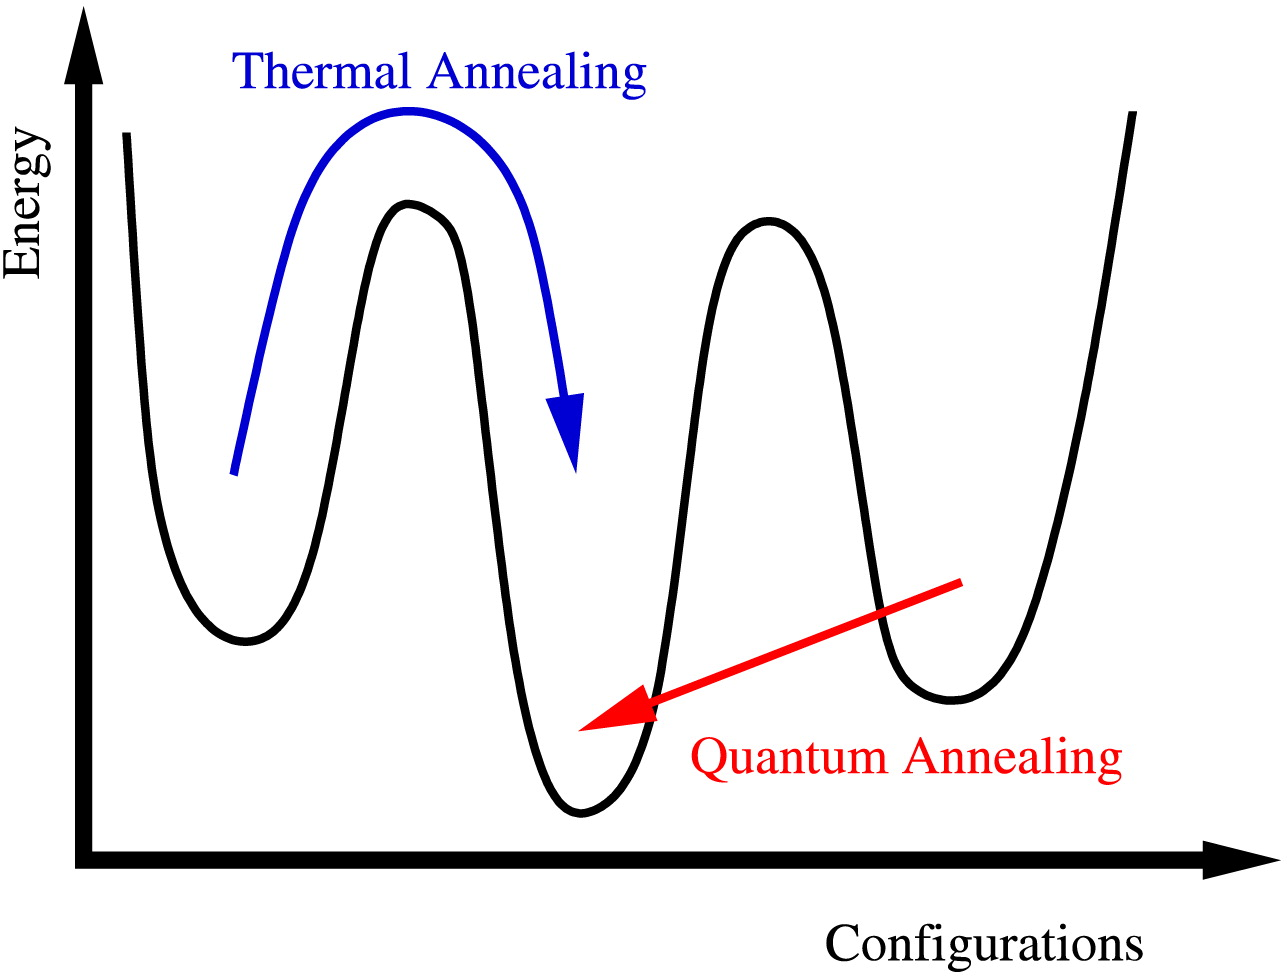
\includegraphics[width = 5cm]{Plots/tunneling.jpg}
      \hspace*{12pt}\hbox{\scriptsize {\footnotesize\itshape \href{https://doi.org/10.1016/j.physrep.2012.10.002}{V. Bapst et al., \textit{Physics Reports} 523 (2013)}}}}
    \end{textblock*}
    \visible<8->{
    \item wähle monoton fallende Funktion für $\Gamma(t)$ (\enquote{ausglühen})}
    \begin{itemize}
      \visible<9->{\item $\lim_{t \to \infty} \Gamma (t) = 0$ \textrightarrow $\lim_{t \to \infty} H(t) = H_\text{f}$}
    \end{itemize}
  \end{itemize} 
\end{frame}  

\begin{frame}{Adiabatische Zeit}
  \visible<1->{}
  \visible<2->{\begin{block}{Adiabatisches Theorem der Quantenmechanik}
    \begin{center}
     System bleibt im selben Eigenzustand von $H$, wenn sich $H$ hinreichend langsam ändert 
    \end{center}    
  \end{block}}
  \vspace*{0.5cm}
   \begin{itemize}
    \setlength\itemsep{1em}
    \visible<3->{
    \item minimale Zeit, damit sich System adiabatisch ändert $\tau$}
    \visible<4->{\item $\symup{\Delta} (t) = E_1 (t) - E_0 (t)$ }
    \visible<5->{
    \item mindestens $\tau \propto \frac{1}{\symup{\Delta} (t)^2}$, schlimmstenfalls $\tau \propto \frac{1}{\symup{\Delta} (t)^3}$ }
    \visible<6->{\item Problem: $\symup{\Delta} (t)$ sehr klein }
    \begin{itemize}
      \visible<7->{\item[\textrightarrow] $\tau \to \infty$}
    \end{itemize}
   \end{itemize}
   \begin{textblock*}{5cm}(8cm, 5cm) % {block width} (coords)
    \visible<4->{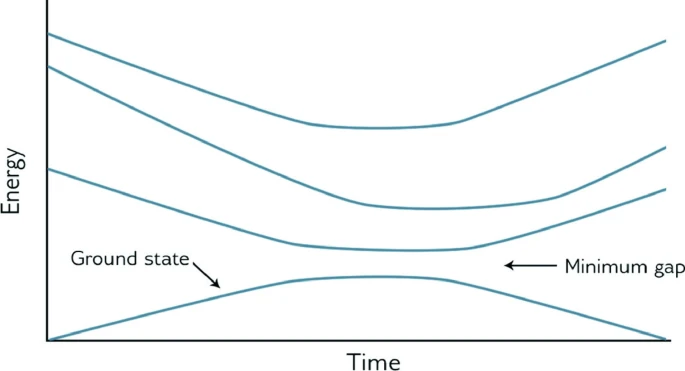
\includegraphics[width = 6.5cm]{Plots/gap.png}
    \hspace*{12pt}\hbox{\scriptsize {\footnotesize\itshape \href{https://link.springer.com/chapter/10.1007/978-3-031-13909-3_14}{E. R. Miranda (Ed.), Quantum Computer Music (2022)}}}}
  \end{textblock*}

\end{frame}

\begin{frame}{Simulation zu simulated und quantum annealing}
\begin{textblock*}{5cm}(10cm, 1.5cm) % {block width} (coords)
  \visible<1->{\begin{equation*}
  {H (t) = \underbrace{- \sum_{ij} J_{ij} \sigma_i^z \sigma_j^z - h \sum_i \sigma_i^z }_{H_\text{f}} \underbrace{- \Gamma (t) \sum_i \sigma_i^x}_{H_\text{i}(t)}}
  \end{equation*}}
\end{textblock*}
  \visible<2->{
  \begin{itemize}
    \item $P_\text{SA}(t)$: Wahrscheinlichkeit System in GZ zu finden
    \item $P_\text{QA}(t)$ = $|\braket{g}{\Psi(t)}|^2$: Wahrscheinlichkeit System in GZ $\ket{g}$ von $H_\text{f}$ zu finden
    \item $P_\text{SA}^{\text{st}}(T)$: Boltzmann-Faktor des GZ von $H_\text{f}$
    \item $P_\text{QA}^{\text{st}}(\Gamma) = | \braket{g}{\Psi_{\Gamma}} |^2$ mit $\ket{\Psi_{\Gamma}}$ als GZ von $H$}
    \visible<3->{\item $\lim_{t \to 0} \Gamma(t) = \lim_{t \to 0} T(t) = \infty$}
    \begin{itemize}
      \visible<4->{\item[\textrightarrow] Superposition aller Zustände gleicher Amplitude (QA)
      \item[\textrightarrow] Alle Zustände gleich wahrscheinlich (SA) }
    \end{itemize}
    \visible<5->{\item Idealfall (adiabatisch): $\lim_{t \to \infty} P_\text{QA}(t) = \lim_{t \to \infty} P_\text{SA}(t) = 1$}
    \begin{itemize}
      \visible<6->{\item[\textrightarrow] Grundzustand gefunden}
      \visible<7->{\item[\textrightarrow] sonst: In einem lokalen Minimum \enquote{hängen} geblieben }
    \end{itemize}
    \visible<8->{\item 8 Spins} 
  \end{itemize}
  \begin{textblock*}{5cm}(10cm, 4.2cm) % {block width} (coords)
    \visible<7->{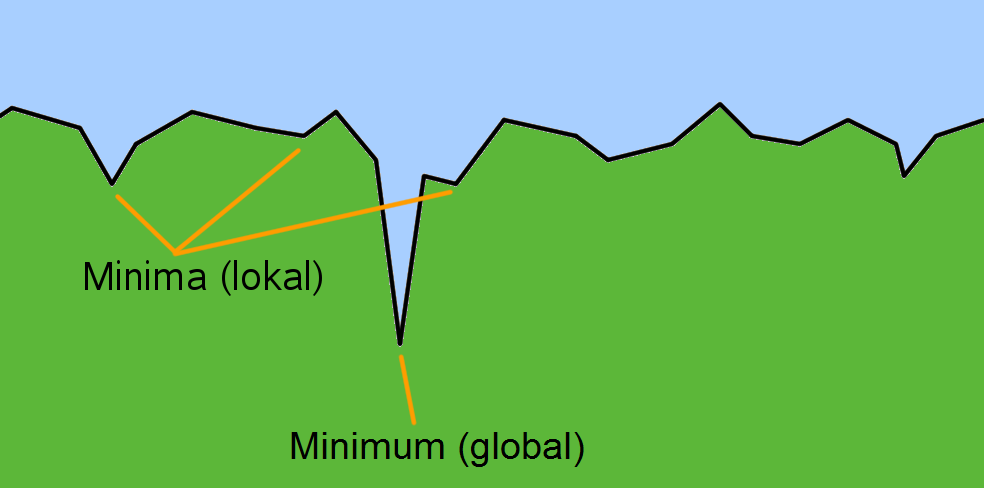
\includegraphics[width = 5.2cm]{Plots/SimAnnealingLandschaft.png}
    \hspace*{12pt}\hbox{\scriptsize {\footnotesize\itshape \href{https://de.wikipedia.org/wiki/Simulated_Annealing}{Fleischer, K., wikipedia.org}}}}
  \end{textblock*}
  \begin{textblock*}{5cm}(0.5cm, 9cm)
    {\footnotesize \href{https://arxiv.org/abs/cond-mat/9804280}{Kadowaki, T., Nishimori, H., \textit{PHYSICAL REVIEW E } 1998}}
  \end{textblock*}
    
\end{frame}

\begin{frame}{Ergebnisse zu simulated und quantum annealing}
  \vspace*{-2.5cm}
  \begin{itemize}
    \item $P_\text{SA}(t)$: Wahrscheinlichkeit System in GZ zu finden
    \item $P_\text{QA}(t)$ = $|\braket{g}{\Psi(t)}|^2$: Wahrscheinlichkeit System in GZ $\ket{g}$ von $H_\text{f}$ zu finden
    \item $P_\text{SA}^{\text{st}}(T)$: Boltzmann-Faktor des GZ von $H_\text{f}$
    \item $P_\text{QA}^{\text{st}}(\Gamma) = | \braket{g}{\Psi_{\Gamma}} |^2$ mit $\ket{\Psi_{\Gamma}}$ als GZ von $H$
  \end{itemize}
  \begin{textblock*}{3cm}(10.2cm, 1.8cm)
  \fbox{\parbox{\textwidth}{
    \begin{itemize}
    \item $J_{ij}  = const > 0$
    \item $h = 0.1$
    \end{itemize}}}
  \end{textblock*}
  \begin{textblock*}{7.5cm}(7.7cm, 3.5cm) % {block width} (coords)
  \begin{center}
    {\color{tugreen}
    $\Gamma(t) = T(t) = 3/ \ln (t+1)$ }
  \end{center}
    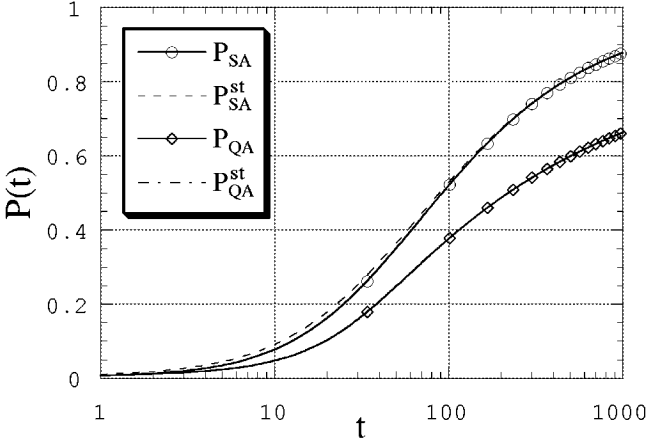
\includegraphics[width = 7.5cm]{Plots/ln.png}
    \end{textblock*}
    \begin{textblock*}{5cm}(0.5cm, 9cm)
      {\footnotesize \href{https://arxiv.org/abs/cond-mat/9804280}{Kadowaki, T., Nishimori, H., \textit{PHYSICAL REVIEW E } 1998}}
    \end{textblock*}
    \begin{textblock*}{3.5cm}(1.7cm, 5.3cm)
      \centering
      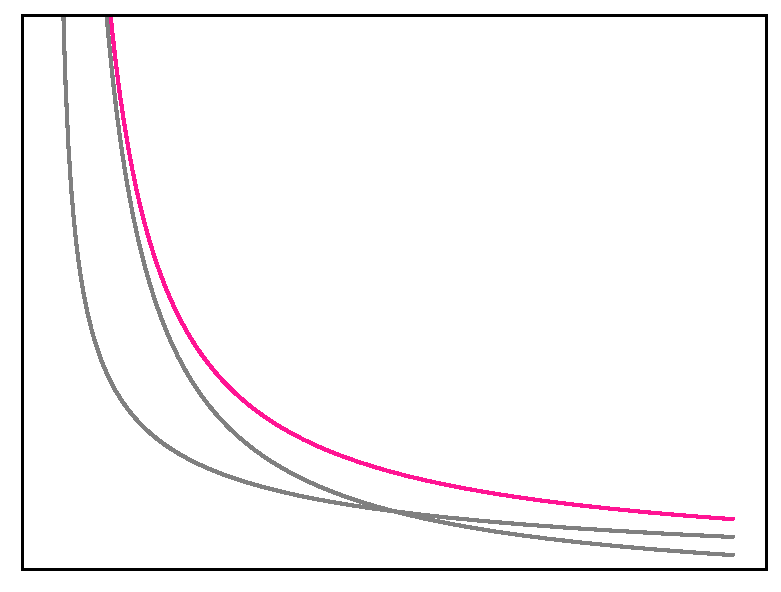
\includegraphics[width = 4.5cm]{Plots/ln.pdf}
    \end{textblock*}
\end{frame}

\begin{frame}{Ergebnisse zu simulated und quantum annealing}
  \vspace*{-2.5cm}
  \begin{itemize}
    \item $P_\text{SA}(t)$: Wahrscheinlichkeit System in GZ zu finden
    \item $P_\text{QA}(t)$ = $|\braket{g}{\Psi(t)}|^2$: Wahrscheinlichkeit System in GZ $\ket{g}$ von $H_\text{f}$ zu finden
    \item $P_\text{SA}^{\text{st}}(T)$: Boltzmann-Faktor des GZ von $H_\text{f}$
    \item $P_\text{QA}^{\text{st}}(\Gamma) = | \braket{g}{\Psi_{\Gamma}} |^2$ mit $\ket{\Psi_{\Gamma}}$ als GZ von $H$
  \end{itemize}
  \begin{textblock*}{3cm}(10.2cm, 1.8cm)
  \fbox{\parbox{\textwidth}{
    \begin{itemize}
    \item $J_{ij}  = const > 0$
    \item $h = 0.1$
    \end{itemize}}}
  \end{textblock*}
  \begin{textblock*}{7.5cm}(7.7cm, 3.5cm) % {block width} (coords)
  \begin{center}
    {\color{tugreen}
    $\Gamma(t) = T(t) = 3/ \sqrt{t}$ }
  \end{center}
    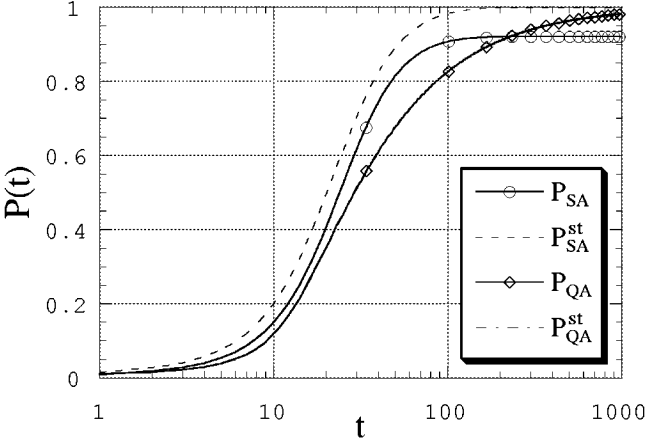
\includegraphics[width = 7.5cm]{Plots/sqrt.png}
    \end{textblock*}
    \begin{textblock*}{5cm}(0.5cm, 9cm)
      {\footnotesize \href{https://arxiv.org/abs/cond-mat/9804280}{Kadowaki, T., Nishimori, H., \textit{PHYSICAL REVIEW E } 1998}}
    \end{textblock*}
    \begin{textblock*}{3.5cm}(1.7cm, 5.3cm)
      \centering
      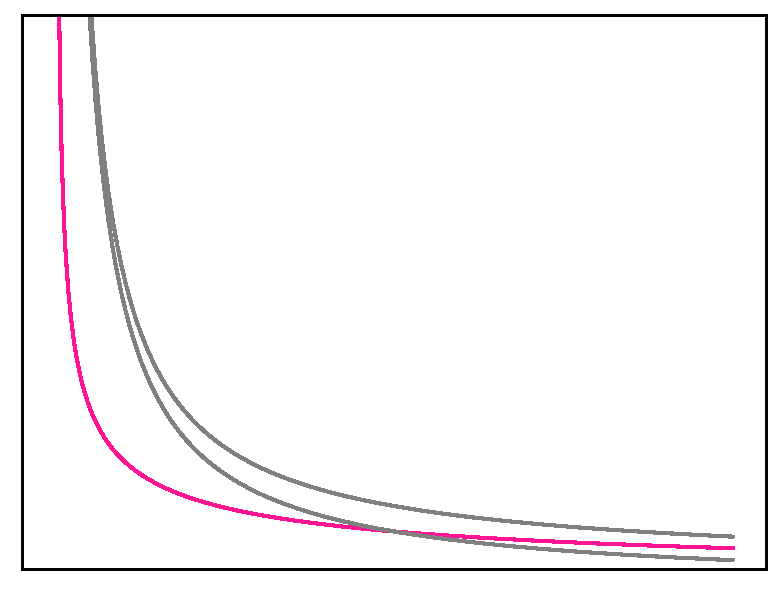
\includegraphics[width = 4.5cm]{Plots/sqrt.pdf}
    \end{textblock*}
\end{frame}

\begin{frame}{Ergebnisse zu simulated und quantum annealing}
  \vspace*{-2.5cm}
  \begin{itemize}
    \item $P_\text{SA}(t)$: Wahrscheinlichkeit System in GZ zu finden
    \item $P_\text{QA}(t)$ = $|\braket{g}{\Psi(t)}|^2$: Wahrscheinlichkeit System in GZ $\ket{g}$ von $H_\text{f}$ zu finden
    \item $P_\text{SA}^{\text{st}}(T)$: Boltzmann-Faktor des GZ von $H_\text{f}$
    \item $P_\text{QA}^{\text{st}}(\Gamma) = | \braket{g}{\Psi_{\Gamma}} |^2$ mit $\ket{\Psi_{\Gamma}}$ als GZ von $H$
  \end{itemize}
  \begin{textblock*}{3cm}(10.2cm, 1.8cm)
  \fbox{\parbox{\textwidth}{
    \begin{itemize}
    \item $J_{ij}  = const > 0$
    \item $h = 0.1$
    \end{itemize}}}
  \end{textblock*}
  \begin{textblock*}{7.5cm}(7.7cm, 3.5cm) % {block width} (coords)
  \begin{center}
    {\color{tugreen}
    $\Gamma(t) = T(t) = 3/t$ }
  \end{center}
    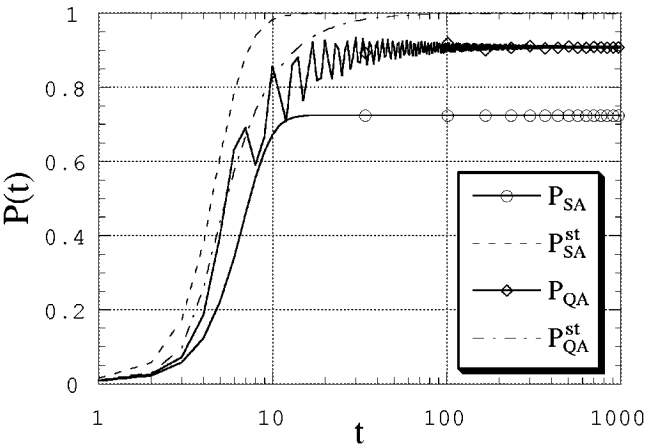
\includegraphics[width = 7.5cm]{Plots/t.png}
    \end{textblock*}
    \begin{textblock*}{5cm}(0.5cm, 9cm)
      {\footnotesize \href{https://arxiv.org/abs/cond-mat/9804280}{Kadowaki, T., Nishimori, H., \textit{PHYSICAL REVIEW E } 1998}}
    \end{textblock*}
    \begin{textblock*}{3.5cm}(1.7cm, 5.3cm)
      \centering
      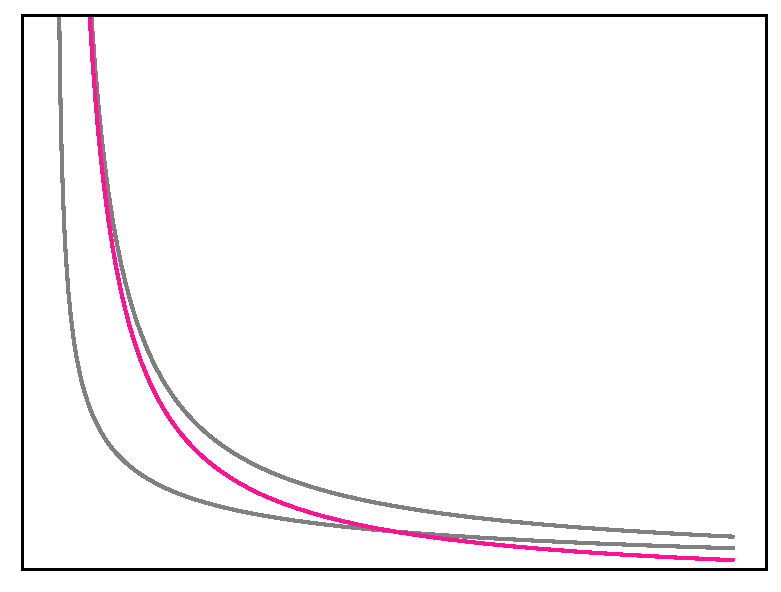
\includegraphics[width = 4.5cm]{Plots/t.pdf}
    \end{textblock*}
\end{frame}

\section{Quadratic unconstrained binary optimization}

\begin{frame}{Binäre Variable}
  \pause
  \begin{itemize}
    \item $x \in \{0,1\}$ \pause
  \end{itemize}
  \vspace*{0.4cm}
  \underline{Beispiel: Aufenthaltsort von einem Truck}
  \begin{itemize}
    \setlength\itemsep{1em}
    \item Formulierung als Graph mit $N$ Knoten $i$ \pause
    \item ordne jedem Knoten $i$ eine binäre Variable zu \pause
    \item jedem Truck kann ein Vektor $x^j = (x^j_1, \ldots, x^j_N)$ von binären Variablen zugeordnet werden  \pause
    \item Truck $j$ an Knoten $i$ \textrightarrow $x^j_i = 1$ sonst $x^j_k = 0$ 
    \end{itemize}
\end{frame}

\begin{frame}{Binäre Variable}
  \begin{columns}
    \column{0.7 \textwidth}
      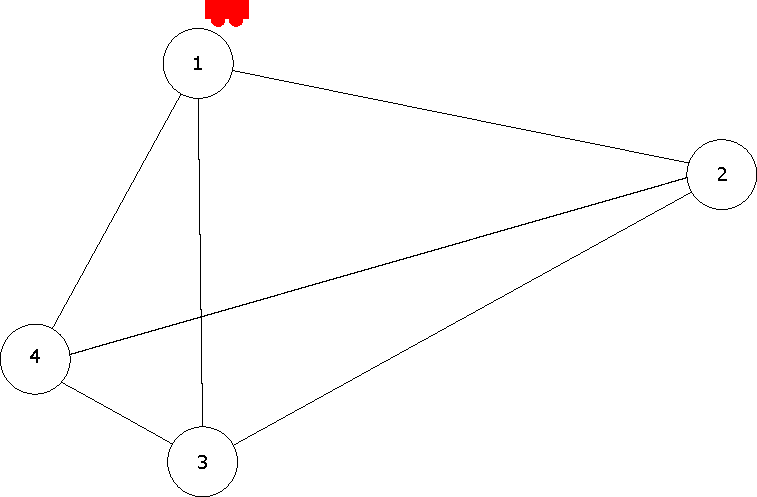
\includegraphics[width = \textwidth]{Plots/binary_1.pdf}
    \column{0.3 \textwidth}
  \begin{myequation}
    \underline{x}^\text{rot} \; \; = 
    \begin{pmatrix}
      1 \\ 0 \\ 0 \\ 0
    \end{pmatrix}
  \end{myequation}
  \end{columns}
\end{frame}

\begin{frame}{Binäre Variable}
  \begin{columns}
    \column{0.7 \textwidth}
      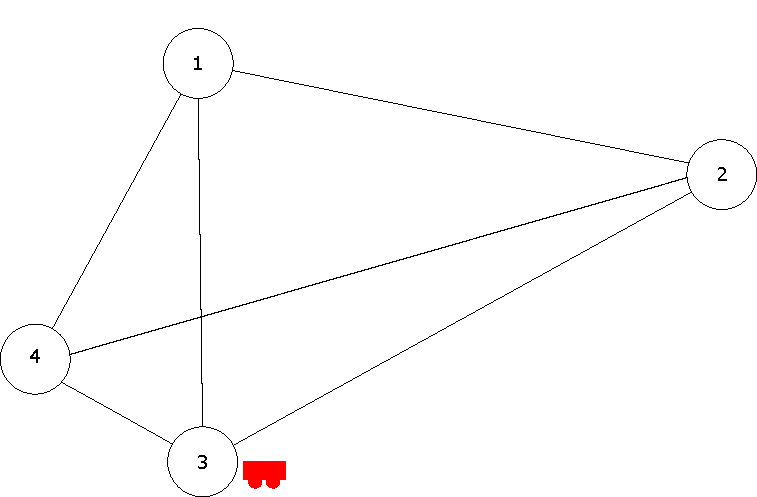
\includegraphics[width = \textwidth]{Plots/binary_2.pdf}
    \column{0.3 \textwidth}
  \begin{myequation}
    \underline{x}^\text{rot} \; \; = 
    \begin{pmatrix}
      0 \\ 0 \\ 1 \\ 0
    \end{pmatrix}
  \end{myequation}
  \end{columns}
\end{frame}

\begin{frame}{Binäre Variable}
  \begin{columns}
    \column{0.7 \textwidth}
      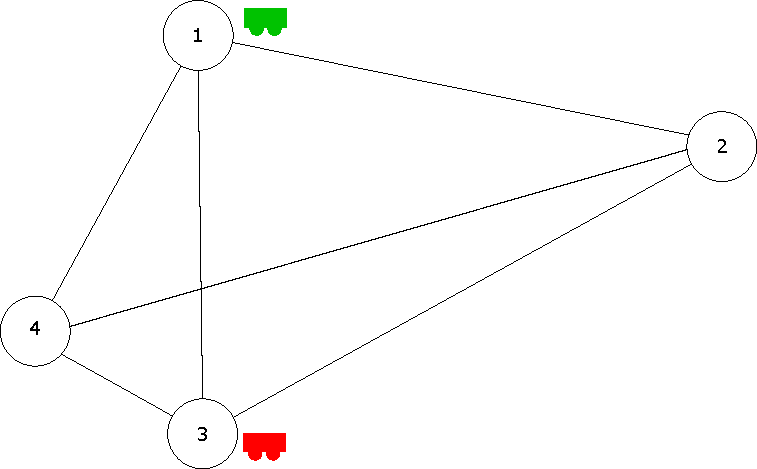
\includegraphics[width = \textwidth]{Plots/binary_3.pdf}
    \column{0.3 \textwidth}
  \begin{myequation}
    \underline{x}^\text{rot} \; \;  = 
    \begin{pmatrix}
      0 \\ 0 \\ 1 \\ 0
    \end{pmatrix}
  \end{myequation}
  \begin{myequation}
    \underline{x}^\text{grün} = 
    \begin{pmatrix}
      1 \\ 0 \\ 0 \\ 0
    \end{pmatrix}
  \end{myequation}
  \end{columns}
\end{frame}

\begin{frame}{Binäre Variable}
  \begin{columns}
    \column{0.7 \textwidth}
      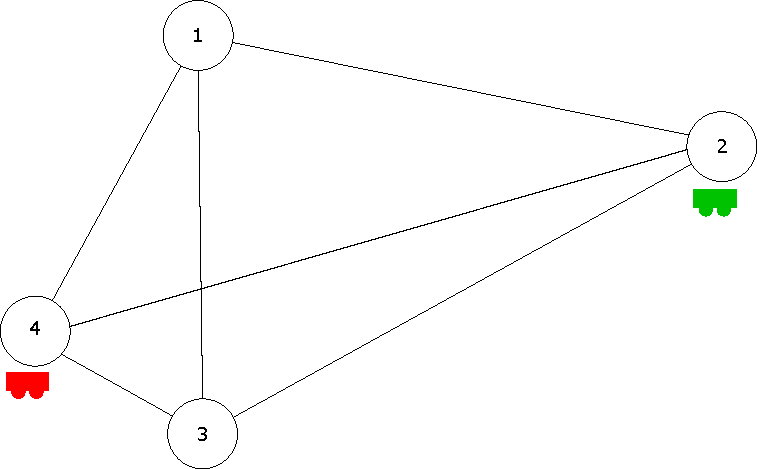
\includegraphics[width =  \textwidth]{Plots/binary_4.pdf}
    \column{0.3 \textwidth}
  \begin{myequation}
    \underline{x}^\text{rot} \; \;  = 
    \begin{pmatrix}
      0 \\ 0 \\ 0 \\ 1
    \end{pmatrix}
  \end{myequation}
  \begin{myequation}
    \underline{x}^\text{grün} = 
    \begin{pmatrix}
      0 \\ 1 \\ 0 \\ 0
    \end{pmatrix}
  \end{myequation}
  \end{columns}
\end{frame}

\begin{frame}{Quadratic unconstrained binary optimization (QUBO)} \pause
  \begin{block}{Aufgabe}
    \center
     Minimiere $ f(\underline{x}, \underline{\underline{Q}}) = \sum_{ij} Q_{ij} x_ix_j$ \pause
  \end{block}
  \begin{itemize}
    \setlength\itemsep{1em}
    \item $Q_{ij}$ definiert Wechselwirkung zwischen $x_i$ \pause
    \begin{itemize}
      \item allg. hermitesch (symmetrisch im Ising-Modell)
    \end{itemize}
    \item $x_i \in \{0,1\}$ als binäre Variable \pause
    \begin{itemize}
      \item lässt sich mittels $s_i = 2x_i - 1 \in \{-1, 1\}$ auf Ising-Variablen (\enquote{Spin-1/2}) transformieren \pause
    \end{itemize}
  \end{itemize}
\end{frame}
 
\begin{frame}{Quadratic unconstrained binary optimization constraints}
  \visible<1->{}
  \begin{itemize}
    \visible<2->{
    \item constraints lassen sich nicht direkt in der Hardware implementieren }
    \begin{itemize}
      \visible<3->{\item[\textrightarrow] constraints als \enquote{Strafe} in der Kostenfunktion implementieren}
    \end{itemize}
    \visible<4->{\item Beispiel: Ein Truck darf sich nur an einem Punkt aufhalten}
    \begin{itemize} 
      \visible<5->{\item $\sum_{i} x_i = 1 \iff \sum_i x_i - 1 = 0$}
      \visible<6->{\item in QUBO-Problem umwandeln \textrightarrow $g = (\sum_i x_i - 1)^2 $}
      \visible<7->{\item[\textrightarrow] $f \to f + \lambda g$ }
      \visible<8->{\item constraint verletzt \textrightarrow Kostenfunktion erhöht}
    \end{itemize}
    \visible<9->{\item Lagrangeparameter $\lambda$ sehr groß wählen}
    \begin{itemize}
      \visible<10->{\item[\textrightarrow] constraint eingehalten}
    \end{itemize} 
  \end{itemize}
  \begin{textblock*}{6.5cm}(9cm, 4.3cm)
    \centering
    \visible<4->{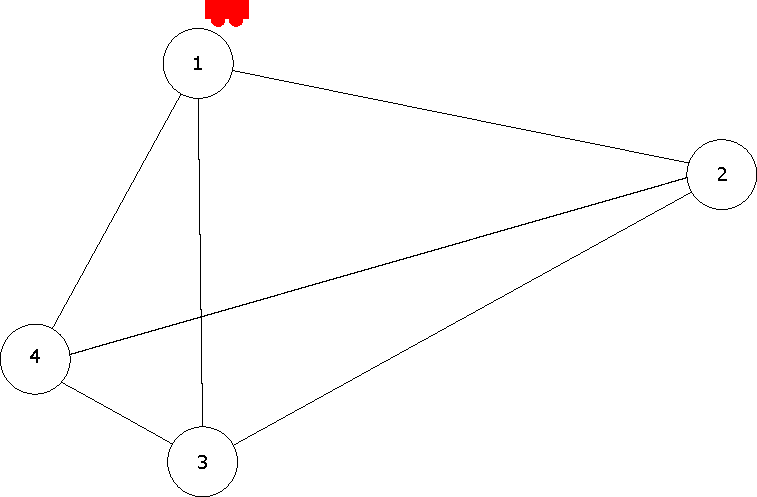
\includegraphics[width = \textwidth]{Plots/binary_1.pdf}}
  \end{textblock*}
\end{frame}

\section{Hardware embedding}

\begin{frame}{Quantum annealer von D-Wave Systems}
  \begin{itemize}
    \item D-Wave Systems als Hersteller von quantum annealer \pause
    \item Qantum Processing Unit (QPU) mit qubits und coupler \pause
    \begin{itemize}
      \item qubits und coupler sind gewichtet  \pause
    \end{itemize}
    \item neuste Version: 5000 qubits mit 15 coupler pro qubit \pause 
    \item Nach annealing-Prozess die qubits auslesen \pause
    \begin{itemize}
      \item[\textrightarrow] mögliches Energieminimum gefunden \pause
    \end{itemize}
  \end{itemize}
  \vspace*{1cm} 
  \underline{Unterschied zu Quantencomputer} \pause
    \begin{itemize}
      \item Quantum annealer nur für kombinatorische Optimierungsprobleme \pause
      \item Quantencomputer nutzen Quantengatter (unitäre Operationen) \pause
      \begin{itemize}
        \item kann mehr Probleme lösen
      \end{itemize}
    \end{itemize}
  \begin{textblock*}{5cm}(11cm, 2cm) % {block width} (coords)
    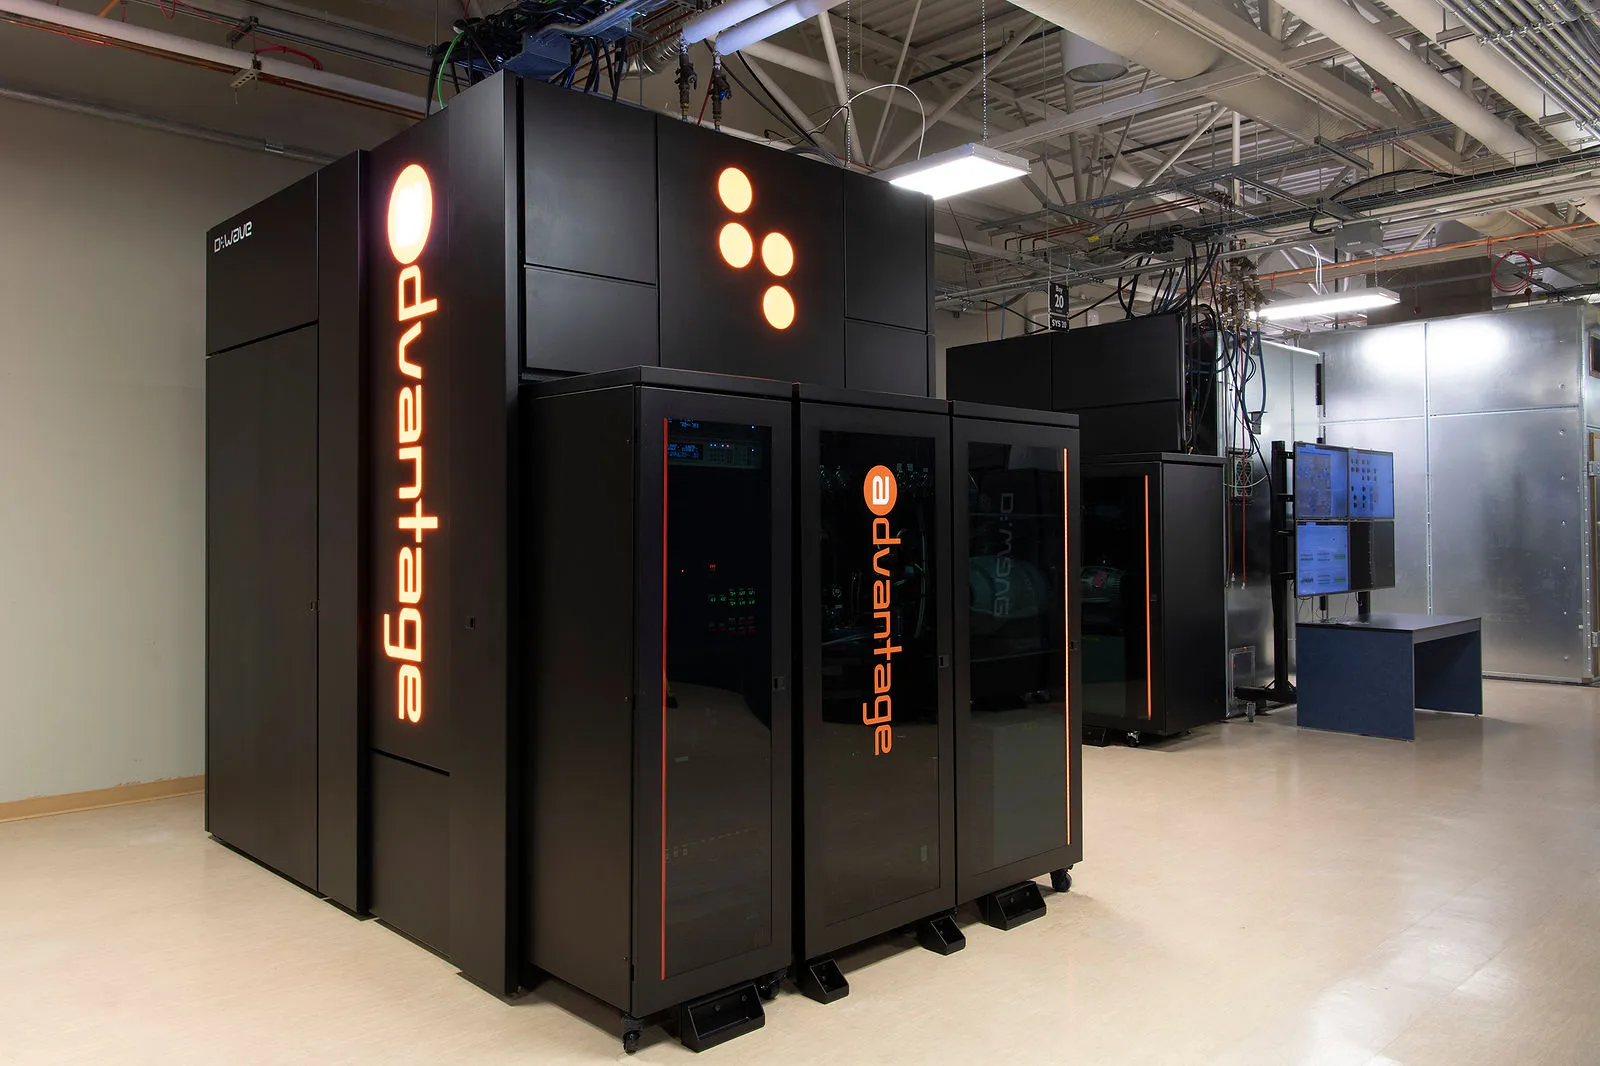
\includegraphics[width = 4.5cm]{Plots/advantage.png}
    \hspace*{12pt}\hbox{\scriptsize {\footnotesize\itshape \href{https://techcrunch.com/2020/09/29/d-wave-launches-its-5000-qubit-advantage-system/?guccounter=1&guce_referrer=aHR0cHM6Ly93d3cuZ29vZ2xlLmNvbS8&guce_referrer_sig=AQAAABB4SLnDOFLkzRsw3QLBP_BiwlTIN9jcs7feoLJi2DljlJifaHVtboTJQonfs2ulmdbT5fTNEU2jmeVP5gqNb_JTbAo88uHq76dEKRkeHYKpmXgEykCXVF3Y_-0ElGKOQqpS-rDrEZJWjMQh3x6OqCY4Pqpfeir7y8_RZCm6FRIW}{techchrunch.com}}}
  \end{textblock*}
  \begin{textblock*}{3cm}(12cm,5.8cm) % {block width} (coords)
    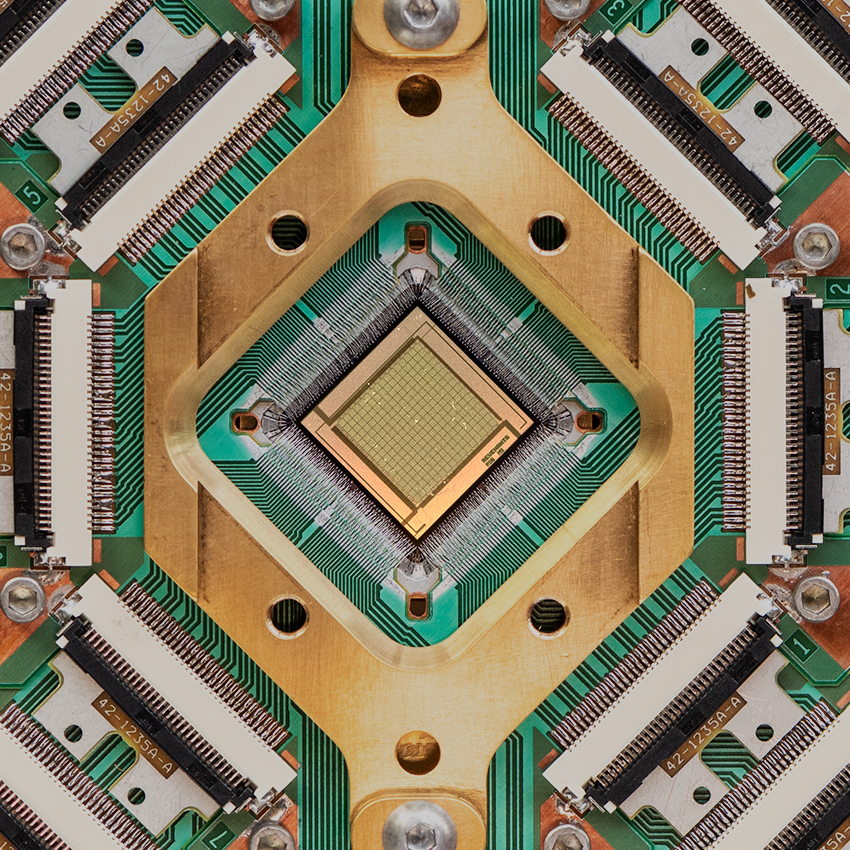
\includegraphics[width = 3cm]{Plots/QPU.jpg}
    \hspace*{12pt}\hbox{\scriptsize {\footnotesize\itshape \href{https://www.dwavesys.com/solutions-and-products/systems/}{dwavesys.com}}}
  \end{textblock*}  
\end{frame}

\begin{frame}{Embedding}
  \visible<1->{}
    \begin{itemize}
    \setlength\itemsep{1em}
    \visible<2->{
    \item D-Wave's QPU kann als Graph $U$ gesehen werden}
    \begin{itemize}
      \visible<3->{
      \item Gewichtete Vertices (qubits) $i \in V(U)$ }
      \visible<4->{
      \item Gewichtete Kanten (coupler) $ij \in E(U)$ }
    \end{itemize}
    \visible<5->{\item Gewichte:
    \begin{itemize}
      \item $h_i (t)$ \enquote{qubit bias}
      \item $\symup{\Delta}_i(t)$ \enquote{tunneling amplitude}
      \item $J_{ij}(t)$ \enquote{coupler strength}
    \end{itemize}}
    \visible<6->{ \item formuliere transversalen Ising-Hamiltonian auf Graph $G$
    \begin{itemize}
      \vspace*{0.1cm}
      \item $H(t) = \sum_{i \in V(G)} h_i(t) \sigma_i^z + \sum_{ij \in E(G)} J_{ij}(t) \sigma_i^z \sigma_j^z + \sum_{i \in V(G)} \Delta_i (t) \sigma_i^x$ }
    \end{itemize}
    \visible<7->{\item Eigenergie des Ising-Hamiltonians $\epsilon(s_1, \ldots, s_n) = \sum_{i \in V(G)} h_i s_i + \sum_{ij \in E(G)} J_{ij} s_i s_j$}
    \begin{itemize}
      \item \visible<8->{ Spins $s_i \in \{-1,1\}$}
    \end{itemize}
    \item \visible<9->{Suche nach Grundzustandsenergie ist das \enquote{Ising-Problem}}
  \end{itemize}
  \begin{textblock*}{5cm}(10.4cm, 3cm) % {block width} (coords)
    \visible<2->{{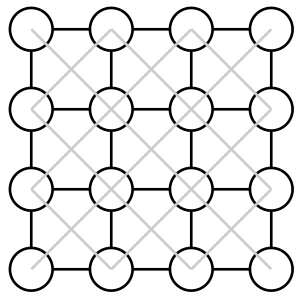
\includegraphics[width = 4.5cm]{Plots/4x4_graph.png}}}
  \end{textblock*}  
  \begin{textblock*}{6cm}(0.5cm, 9cm)
    {\footnotesize \href{https://doi.org/10.1016/j.physrep.2012.10.002}{V. Choi, \textit{D-Wave Systems Inc.} (2008)}}
  \end{textblock*}
\end{frame}

\begin{frame}{Embedding}
  \visible<1->{}
  \begin{textblock*}{5cm}(8.5cm, 2cm) % {block width} (coords)
    \visible<2->{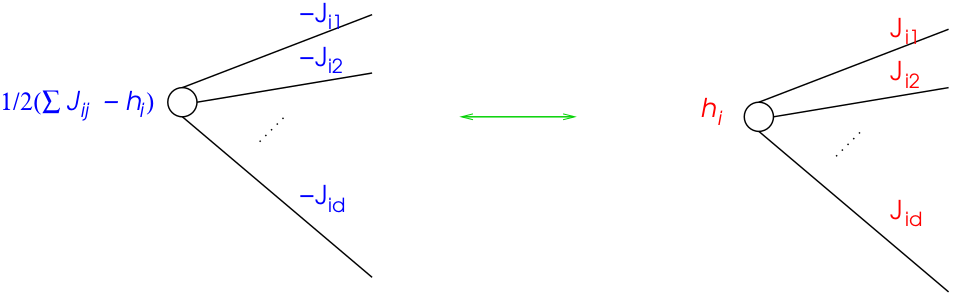
\includegraphics[width = 7cm]{Plots/qubo_ising_rev.png}}
  \end{textblock*}
   \begin{itemize}
   \visible<2->{ \item Ising- äquivalent zu QUBO-Problem auf dem selben Graph $G$ }
    \begin{itemize}
     \visible<3->{ \item $Y(x_1, \ldots, x_n) = \sum_{i \in V(G)} c_i x_i - \sum_{ij \in E(G)} J_{ij} x_i x_j $ maximieren 
      \item $x_i \in \{0,1\}$ }
    \end{itemize}
  \end{itemize}
  \visible<4->{\begin{block}{Ziel}
       $G$ in $U$ einbetten (\enquote{subgraph-embedding}) und somit das Ising/QUBO-Problem lösen
    \end{block}}
    \begin{itemize}
      \visible<5->{\item Problem: Einschränkungen durch Anzahl der coupler auf $U$ übertragen sich auf $G$}
      \begin{itemize}
        \visible<6->{\item[\textrightarrow] \enquote{dummy}-Vertices mit ferromagnetischer Kopplung einführen}
      \end{itemize}
    \end{itemize}
    \begin{textblock*}{2cm}(12cm, 6.6cm) % {block width} (coords)
      \visible<5->{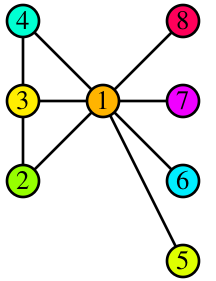
\includegraphics[width =2cm]{Plots/grap_g.png}}
    \end{textblock*}
    \begin{textblock*}{6cm}(0.5cm, 9cm)
      {\footnotesize \href{https://doi.org/10.1016/j.physrep.2012.10.002}{V. Choi, \textit{D-Wave Systems Inc.} (2008)}}
    \end{textblock*}
\end{frame}

\begin{frame}{Minor embedding}
  \vspace*{1cm}
  \visible<1->{}
  \begin{itemize}
  \visible<2->{\item logischer qubit $i$ aus $G$ wird auf subtree $T_i$ physischer qubits aus $G_\text{emb} \subset U$ abgebildet}
  \item \visible<3->{ ferromagnetische Kopplung zwischen \enquote{dummy}-Vertices muss hinreichend groß sein}
  \end{itemize}
  \vspace*{1cm} \visible<4->{
  \begin{varblock}[6.4cm]{Ziel}
    Parameter des minor-embedding auf ursprüngliche Ising/QUBO-Parameter zurückführen
  \end{varblock}}
  \vspace*{4cm}
  \begin{textblock*}{6cm}(8.5cm, 4.5cm) % {block width} (coords)
    \visible<1->{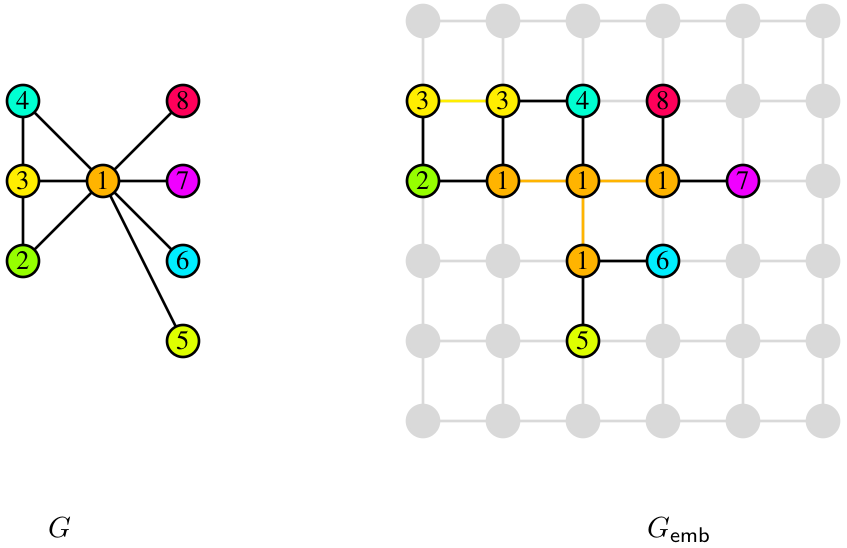
\includegraphics[width = 6.5cm]{Plots/G_emb.png}}
  \end{textblock*}
  \begin{textblock*}{6cm}(0.5cm, 9cm)
    {\footnotesize \href{https://doi.org/10.1016/j.physrep.2012.10.002}{V. Choi, \textit{D-Wave Systems Inc.} (2008)}}
  \end{textblock*}
\end{frame}

\begin{frame}{Minor embedding}
  \visible<1->{}
  \begin{itemize}
    \visible<2->{\item $\epsilon^\text{emb}(s_1, \ldots, s_N) = \sum_{i \in V(G_\text{emb})} h_i's_i + \sum_{ij \in E(G_\text{emb})} J_{ij}' s_i s_j $ minimieren}
    \visible<3->{\item $\tau : V(G) \times V(G) \to V(U)$, so dass $i_{\tau (i,\,j)} \in V(T_i), \; j_{\tau (j,\,i)} \in V(T_j)$ mit $i_{\tau (i,\,j)} \, j_{\tau (j,\,i)} \in E(U)$ }
    \visible<4->{\item $OE(G_\text{emb}) = \cup_{ij \in E(G)} i_{\tau (i,\,j)} \, j_{\tau (j,\,i)}$ sind ursprüngliche coupler }
    \begin{itemize}
     \visible<5->{ \item[\textrightarrow] $J_{i_{\tau (i,\,j)} \, j_{\tau (j,\,i)}}' = J_{ij}$ für $i_{\tau (i,\,j)} \, j_{\tau (j,\,i)} \in OE(G_\text{emb})$}
    \end{itemize}
    \visible<6->{\item ferromagnetische coupler strength $F_k^{ij}$ für $ij \in E(T_i)$ }
    \visible<7->{\item bias $h_i$ der logischen qubits auf physische qubits verteilen   }
    \begin{itemize}
      \visible<8->{\item[\textrightarrow] $\sum_{i_k \in V(T_i)} h_{i_k}' = h_i$ }
    \end{itemize}
  \end{itemize}\visible<9->{
  \begin{block}{Finale Energie}
    \begin{equation*}
      \epsilon^{\text{emb}}(s_1, \ldots, s_N) = \sum_{i \in V(G)} \left (
        \sum_{i_k \in V(T_i)} h_{i_k}' s_{i_k} + \sum_{i_p i_q \in E(T_i)} F_i^{pq} s_{i_p} s_{i_q} \right ) 
        + \sum_{ij \in E(G)} J_{ij} s_{i_{\tau(i,\,j)}} s_{j_{\tau(j,\,i)}}
    \end{equation*}
  \end{block}}
  \begin{textblock*}{6cm}(11cm, 1.7cm) % {block width} (coords)
    \visible<2->{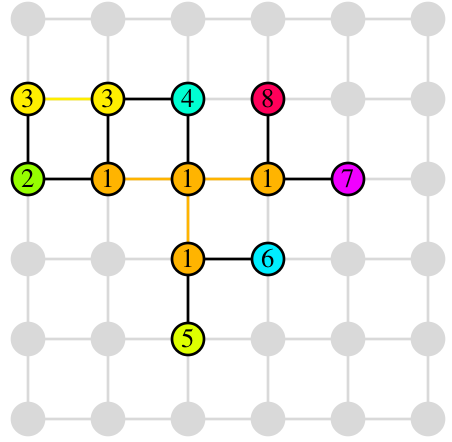
\includegraphics[width = 4cm]{Plots/graph_cut.png}}
  \end{textblock*}
  \begin{textblock*}{6cm}(0.5cm, 9cm)
    {\footnotesize \href{https://doi.org/10.1016/j.physrep.2012.10.002}{V. Choi, \textit{D-Wave Systems Inc.} (2008)}}
  \end{textblock*}
\end{frame}

\section{Fallbeispiel Aisin Corporation}
\begin{frame}{Fallbeispiel Aisin Corporation}
  \begin{textblock*}{5cm}(11cm, 2cm) % {block width} (coords)
    \visible<2->{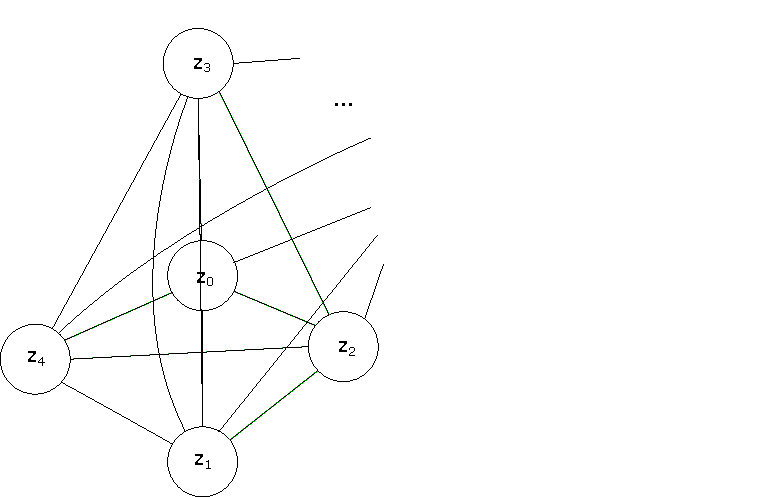
\includegraphics[width = 7cm]{Plots/ex.pdf}}
  \end{textblock*}
  \begin{itemize}
    \visible<3->{\item Zeit für Route $\xi$ : $\text{time}(\xi) = \sum_{t=1}^{k-1} T_{\xi_t, \xi_{t+1}}$ }
    \visible<4->{\item off-board-demand $D_{ij}$, der von $i$ nach $j$ gebracht werden muss              }
  \end{itemize}
  \vspace*{0.3cm}
  \visible<5->{\underline{Terme für QUBO-Formulierung}}
  \begin{itemize}
    \setlength\itemsep{0.7em}
    
    \visible<6->{\item $f_\text{local} (\{ x_i \}) = A_\text{local} \sum_t \left ( 1-\sum_i x_{it} \right )^2$                                                                                                        }    
    \visible<7->{\item $f_\text{time} (\{ x_i \}) = A_\text{time} \sum_{ijt} T_{ij} x_{it}x_{jt+1}$                                                                                                                   }
    \visible<8->{\item $f_\text{demand} (\{ x_i \}) = - A_\text{demand} \sum_{ijt} \sum_{\delta = 1}^{\delta_*(t)} D_{ij} x_{it} x_{j t+\delta}$ mit $\delta_*(t) = \text{min}(\delta_\text{max}, \tau -1 -t)$        }
    \visible<9->{\item $f_\text{nonredundant}^I (\{ x_i \}) = A_{\text{nonredundant}}\sum_{ij} I_{ij} \sum_{\delta = 2}^{\tau - 2} \sum_{t=0}^{\tau - 2 - \delta} x_{it} x_{j t+1} x_{i t+\delta} x_{j t+ 1 +\delta}$ }
    \begin{itemize}
     \visible<10->{ \item Vorsicht: Grad des Polynoms muss noch auf zwei reduziert werden }
    \end{itemize}
    \vspace*{0.5cm}
    \visible<11->{\begin{equation*}
      A_\text{local} = 5000, \quad A_\text{demand} = 320, \quad A_\text{time} = 0.01\quad A_\text{nonredundant} = 1  
    \end{equation*}}
  \end{itemize}

  \begin{textblock*}{6cm}(0.5cm, 9cm)
   \visible<1->{ {\footnotesize \href{https://www.nature.com/articles/s41598-023-31765-8}{Weinberg, S.J., Sanches, F., Ide, T. et al. Sci Rep 13, 4770 (2023)}}}
  \end{textblock*}

\end{frame}

\begin{frame}{Fallbeispiel Aisin Corporation}
  \begin{textblock*}{5cm}(0.5cm, 3cm) % {block width} (coords)
    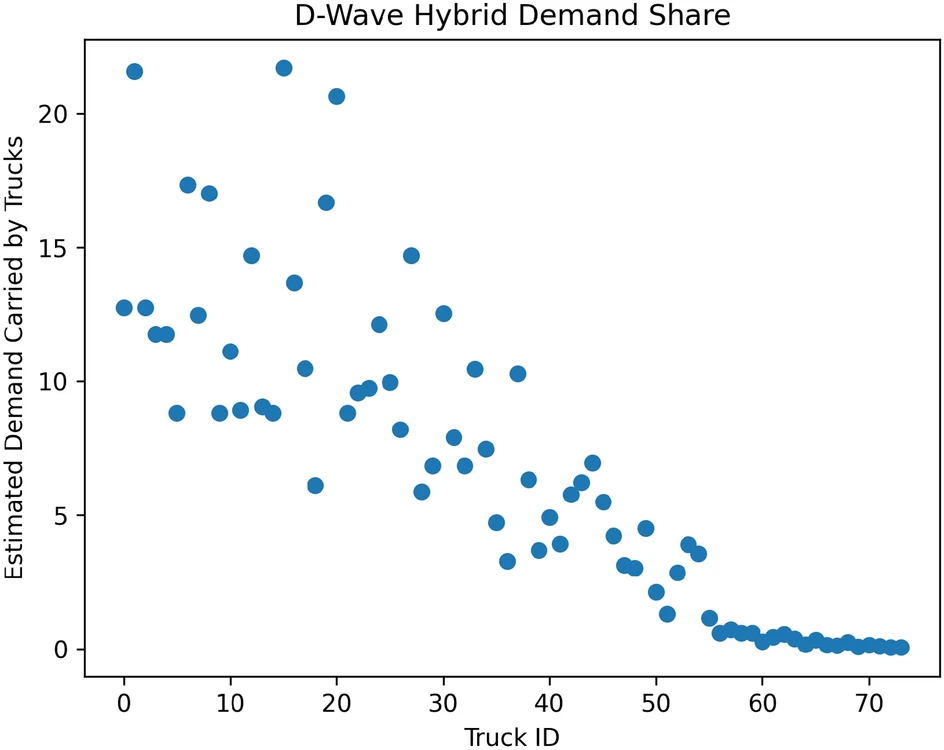
\includegraphics[width = 7cm]{Plots/74.png}
  \end{textblock*}
  \begin{textblock*}{5cm}(8.2cm, 3cm) % {block width} (coords)
    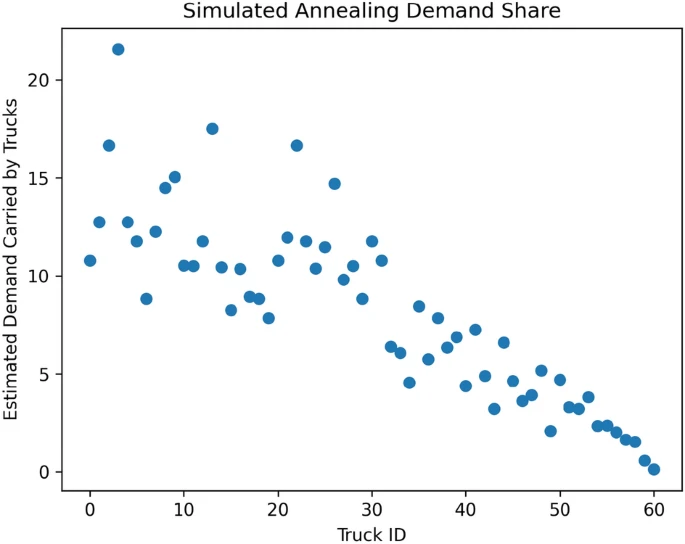
\includegraphics[width = 7cm]{Plots/61.png}
  \end{textblock*}
  \begin{textblock*}{6cm}(0.5cm, 9cm)
    {\footnotesize \href{https://www.nature.com/articles/s41598-023-31765-8}{Weinberg, S.J., Sanches, F., Ide, T. et al. Sci Rep 13, 4770 (2023)}}
  \end{textblock*}
\end{frame}

\begin{frame}{Fallbeispiel Aisin Corporation}
  \begin{textblock*}{5cm}(1cm, 2.5cm) % {block width} (coords)
    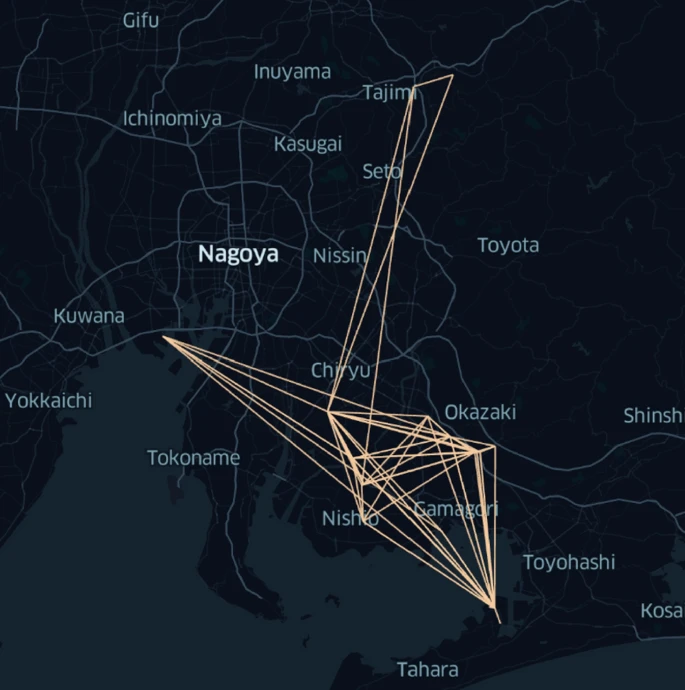
\includegraphics[width = 6cm]{Plots/before.png}
  \end{textblock*}
  \begin{textblock*}{5cm}(9cm, 2.5cm) % {block width} (coords)
    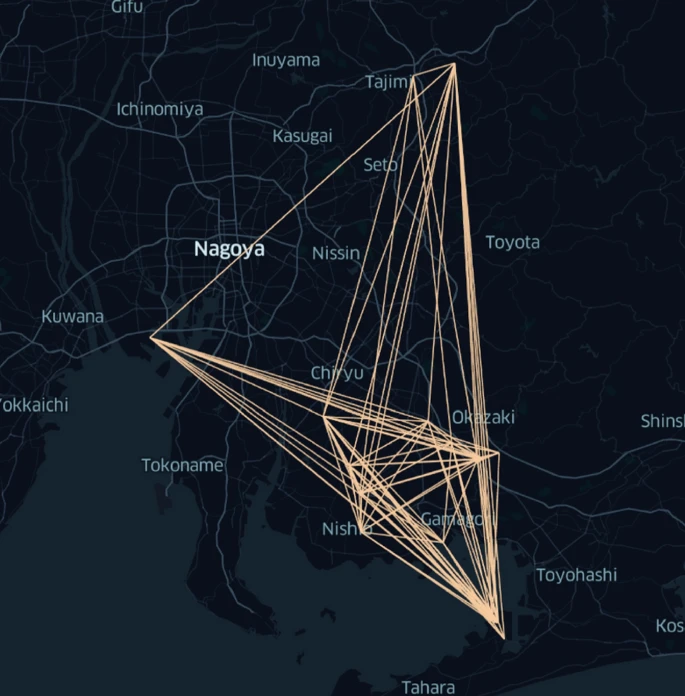
\includegraphics[width = 6cm]{Plots/after.png}
  \end{textblock*}
  \begin{textblock*}{6cm}(0.5cm, 9cm)
    {\footnotesize \href{https://www.nature.com/articles/s41598-023-31765-8}{Weinberg, S.J., Sanches, F., Ide, T. et al. Sci Rep 13, 4770 (2023)}}
  \end{textblock*}
\end{frame}

\section{Zusammenfassung und Ausblick}
\begin{frame}{Zusammenfassung und Ausblick}
  \begin{itemize}[<+(1)->]
    \item QA als heuristische Methode, um Grundzustand zu finden
    \item QA bereits angewandt um Logistik (deutlich) zu verbessern
    \item QA konvergiert wahrscheinlicher als SA
    \item QA und SA nur auf kombinatorische Optimierungsprobleme anwendbar
    \item Komplexität wächst bei QA und SA exponentiell mit Systemgröße
  \end{itemize}
  \vspace*{1cm}
  \pause
  \begin{itemize}
    \item mehr qubits 
    \begin{itemize}
      \item[\textrightarrow] größere Probleme optimieren
    \end{itemize}
    \item mehr coupler
    \begin{itemize}
      \item[\textrightarrow] weniger \enquote{dummy}-Vertices nötig
      \item[\textrightarrow] weniger physische qubits für einen logischen qubit nötig
    \end{itemize}
  \end{itemize}
\end{frame}

\begin{frame}{Quellen}
  \begin{itemize}
    \item Bapst, V. et al., The quantum adiabatic algorithm applied to random optimization
    problems: The quantum Spin glass perspective, \textit{ScienceDirect} 523 (2013), https://doi.org/10.1016/j.physrep.2012.10.002
    \item Kadowaki, T. et al. Quantum annealing in the transverse Ising model,  \textit{PHYSICAL REVIEW E} 58 (1998), https://doi.org/10.48550/arXiv.cond-mat/9804280
    \item Rieffel, E.G., Venturelli, D., O’Gorman, B. et al. A case study in programming a quantum annealer for hard operational planning problems. Quantum Inf Process 14, 1–36 (2015). https://doi.org/10.1007/s11128-014-0892-x
    \item Choi, V. Minor-embedding in adiabatic quantum computation: I. The parameter setting problem. Quantum Inf Process 7, 193–209 (2008). https://doi.org/10.1007/s11128-008-0082-9
    \item Jain, S, Solving the Traveling Salesman
    Problem on the D-Wave Quantum
    Computer, \textit{
      Frontiers in Physics}, Volume 9, id.646 (2021)
 ,doi: 10.3389/fphy.2021.760783
    \item Sangwan, Shabnam. (2018). Literature Review on Travelling Salesman Problem. \textit{International Journal of Research.} 5. 1152. 
    \item Weinberg, S.J., Sanches, F., Ide, T. et al. Supply chain logistics with quantum and classical annealing algorithms. Sci Rep 13, 4770 (2023). https://doi.org/10.1038/s41598-023-31765-8
    \item Yarkoni, S et al., Quantum annealing for industry applications:
    introduction and review, \textit{IOP Publishing} 85-10 (2022), https://dx.doi.org/10.1088/1361-6633/ac8c54
  \end{itemize}
\end{frame}

\begin{frame}{Quellen}
  \begin{itemize}
    \item https://www.dwavesys.com/solutions-and-products/systems/
    \item 
    https://techhq.com/2023/05/industrial-applications-of-quantum-computing-add-up-for-dwave/
    \item https://www.science.org/content/article/quantum-or-not-controversial-computer-runs-no-faster-normal-one
  \end{itemize}
\end{frame}

\begin{frame}{Backup-Folien für Detailfragen}
\centering
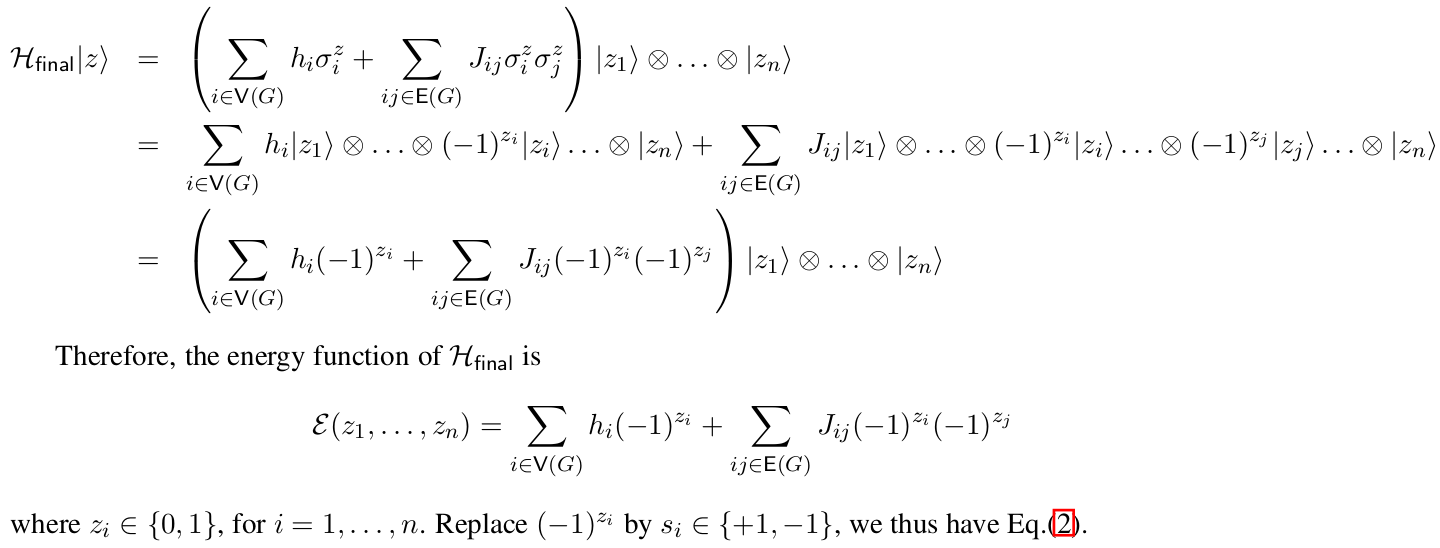
\includegraphics[width = \textwidth]{Plots/ising_energy.png}
\end{frame}

\begin{frame}{Backup-Folien für Detailfragen}
\centering
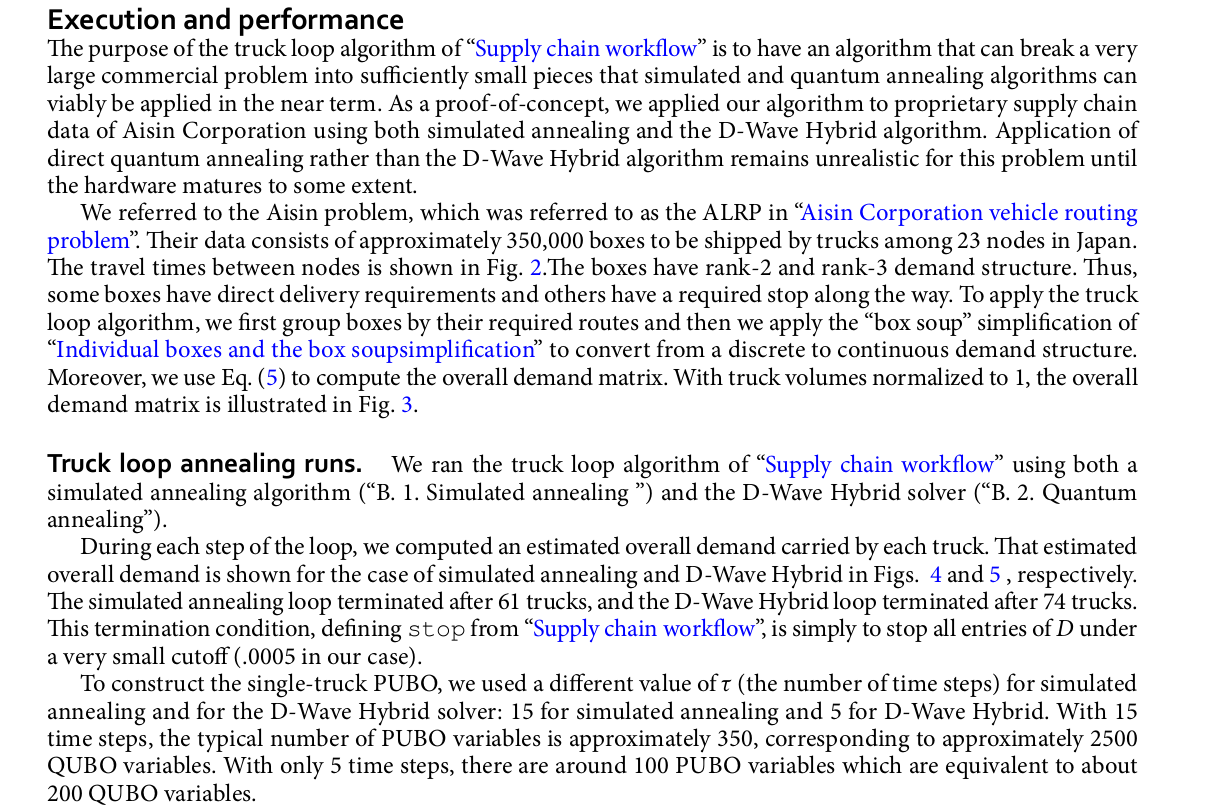
\includegraphics[width = 0.7\textwidth]{Plots/perf.png}
  \end{frame}
\begin{frame}{Backup-Folien für Detailfragen}
  or both the simulated annealing routes and the D-Wave Hybrid routes, we kept only the first 61 trucks. We
found that these trucks satisfied 96.45 percent of the overall Aisin Corp. demand when using simulated annealing and
99.39 percent with the D-Wave Hybrid solver.
\end{frame}

\begin{frame}{Kritik}
  \begin{itemize}
    \item QA skaliert mit Systemgröße wie normaler Computer
    \item Rechenzeit sollte bei Quantencomputer mit Systemgröße langsamer als bei normalen Computer skalieren
    \item In particular, a full-fledged "universal" quantum computer should be able to factor huge numbers ever faster than an ordinary computer as the size of the numbers grow.
    \item Daniel Lidar (University of Southern California in Los Angeles) hat random WW zw. qubits simuliert und gemerkt, dass das Problem exponentiell mit 
    Systemgröße wächst wie bei normalem Computer 
    \item Texas A und M's Katzgraber sagt aber, dass GZ bei random WW typischerweise nur bei T = 0 erreicht werden kann und die Tests somit sinnlos sind
    \item Hartmut Neven, director of engineering at Google, sagt, dass es Klassen von Problemem gibt, wo ein next-generation quantum annealer jeglichen klassischen Algorithmus schlagen wird
    \item Quelle https://www.science.org/content/article/quantum-or-not-controversial-computer-runs-no-faster-normal-one

  \end{itemize}
\end{frame}

\end{document}